\documentclass[11pt]{article}
\usepackage{enumerate}
\usepackage{fullpage}
\usepackage{fancyhdr}
\usepackage{amsmath, amsfonts, amsthm, amssymb}
\usepackage{graphicx}
\usepackage{wasysym}
\setlength{\parindent}{0pt}
\setlength{\parskip}{5pt plus 1pt}
\pagestyle{empty}

\def\indented#1{\list{}{}\item[]}
\let\indented=\endlist

\newcounter{questionCounter}
\newcounter{partCounter}[questionCounter]
\newenvironment{question}[2][\arabic{questionCounter}]{%
    \setcounter{partCounter}{0}%
    \vspace{.25in} \hrule \vspace{0.5em}%
        \noindent{\bf #2}%
    \vspace{0.8em} \hrule \vspace{.10in}%
    \addtocounter{questionCounter}{1}%
}{}
\renewenvironment{part}[1][\alph{partCounter}]{%
    \addtocounter{partCounter}{1}%
    \vspace{.10in}%
    \begin{indented}%
       {\bf (#1)} %
}{\end{indented}}

%%%%%%%%%%%%%%%%%%%%%%%HEADER%%%%%%%%%%%%%%%%%%%%%%%%%%%%%%
\newcommand{\myname}{Shashank Singh\footnote{sss1@andrew.cmu.edu}
        \footnote{Machine Learning Department \& Department of Statistics}}
\newcommand{\myclass}{10-715 Advanced Introduction to Machine Learning}
\newcommand{\myhwnum}{2}
\newcommand{\duedate}{Wednesday October 15, 2014}
%%%%%%%%%%%%%%%%%%%%%%%%%%%%%%%%%%%%%%%%%%%%%%%%%%%%%%%%%%%

%%%%%%%%%%%%%%%%%%%%CONTENT MACROS%%%%%%%%%%%%%%%%%%%%%%%%%
\renewcommand{\qed}{\quad \ensuremath{\blacksquare}}
\newcommand{\inv}{^{-1}}
\newcommand{\bv}{\mathbf{v}}
\newcommand{\bx}{\mathbf{x}}
\newcommand{\by}{\mathbf{y}}
\newcommand{\bff}{\mathbf{f}}
\newcommand{\bzero}{\mathbf{0}}
\newcommand{\bxi}{\boldsymbol{\xi}}
\newcommand{\boldeta}{\boldsymbol{\eta}}
\newcommand{\dist}{\operatorname{dist}}
\newcommand{\area}{\operatorname{area}}
\newcommand{\vspan}{\operatorname{span}}
\newcommand{\Gr}{\operatorname{Gr}} % graph of a function
\renewcommand{\sp}{\operatorname{span}} % span of a set
\newcommand{\sminus}{\backslash}
\newcommand{\E}{\mathbb{E}} % expected value
\newcommand{\F}{\mathcal{F}}
\renewcommand{\H}{\mathcal{H}}
\newcommand{\pr}{\mathbb{P}} % probability
\newcommand{\Var}{\operatorname{Var}} % variance
\newcommand{\N}{\mathbb{N}} % natural numbers
\newcommand{\Z}{\mathbb{Z}} % integers
\newcommand{\Q}{\mathbb{Q}} % rational numbers
\newcommand{\R}{\mathbb{R}} % real numbers
\newcommand{\A}{\mathcal{A}}
\newcommand{\B}{\mathcal{B}}
\newcommand{\C}{\mathcal{C}} % compact functions
\newcommand{\K}{\mathbb{K}} % underlying field of a linear space
\newcommand{\Ran}{\mathcal{R}} % range of a linear operator
\newcommand{\Nul}{\mathcal{N}} % null-space of a linear operator
\renewcommand{\L}{\mathcal{L}} % bounded linear functions
\newcommand{\pow}[1]{\mathcal{P}\left(#1\right)} % power set of #1
\newcommand{\e}{\varepsilon} % \varepsilon
\newcommand{\wto}{\rightharpoonup} % weak convergence
\newcommand{\wsto}{\stackrel{*}{\rightharpoonup}} % weak-* convergence
\newcommand{\X}{\mathcal{X}}
\newcommand{\Y}{\mathcal{Y}}
\renewcommand{\P}{\mathbb{P}}   % probability
\newcommand{\ind}{\perp\!\!\!\perp} % independent
%%%%%%%%%%%%%%%%%%%%%%%%%%%%%%%%%%%%%%%%%%%%%%%%%%%%%%%%%%%

\begin{document}
\thispagestyle{plain}

{\Large Homework \myhwnum, Problems 1 and 2} \\
Name: \myname \\
\myclass \\
Due: \duedate

\section{More Regression and Classification (Samy)}
\subsection{Optimal Classification \& Regression}
\begin{enumerate}
\item Note that, $g(x) = 1_{\{\P[Y = 1 | X = x]\}}$, and hence, if
$f(x) \neq g(x)$, then
\[\P_{XY}[Y \neq g(X)]
    \leq 1/2
    \leq \P_{XY}[Y = g(X)]
    \leq \P_{XY}[Y \neq f(X).\]
Since clearly
$\P_{XY}(Y \neq g(X), f(x) = g(X)) = \P_{XY}(Y \neq f(X), f(x) = g(X))$,
\begin{align*}
R(g)
 &  = \P_{XY}(Y \neq g(X), f(x) = g(X))
    + \P_{XY}(Y \neq g(X), f(x) \neq g(X))  \\
 &  \leq \P_{XY}(Y \neq f(X), f(x) = g(X))
    + \P_{XY}(Y \neq f(X), f(x) \neq g(X))
    = R(f). \qed
\end{align*}
\item For any $x \in \X$, since the objective is smooth and convex, for any
$f : \X \to \Y$ minimizing $\E_Y[(Y - f(X))^2 | X = x]$, under certain
regularity conditions on $f$ and the joint distribution of $(X,Y)$,
\[0
    = \frac{d}{df(x)} \E_Y[(Y - f(X))^2 | X = x]
    = 2 \E_Y[f(X) - Y | X = x]
    = 2 f(x) - \E_Y[Y | X = x]
\]
and hence $f(x) = \E_Y[Y | X = x]$. Hence, the Bayes estimator $g$ minimizes
the risk pointwise (i.e., for all $X$, and so it minimizes the expected risk.
\qed
\end{enumerate}

\subsection{Support Vector Regression}
\begin{enumerate}
\item Let $\xi \in \R^n$ defined by $\xi_i := l_\e(w^Tx_i - y_i)$. Then, the
optimization problem can be written
\[\min_{w \in \R^m, \xi \in \R^n}
    \frac12 \|w\|_2^2 + c \sum_{i = 1}^n \xi_i,
    \quad \mbox{ s.t. } \quad
    0 \leq \xi_i, \xi_i + \e - w^Tx_i + y_i, \xi_i + \e + w^Tx_i - y_i
    \quad \mbox{ for } \quad
    i \in [n],
\]
The Lagrangian is
\[L(w,\xi,\alpha,\beta,\gamma)
    = \frac12 \|w\|_2^2 + \sum_{i = 1}^n c\xi_i - \alpha_i\xi_i
                        - \beta_i(\xi_i + \e - w^Tx_i + y_i)
                        - \gamma_i(\xi_i + \e + w^Tx_i - y_i)
\]
If $\hat w$ and $\hat \xi$ minimize the Lagrangian, then
\[0
    = \nabla_w L(w, \hat \xi,\alpha,\beta,\gamma) \big|_{w = \hat w}
    = \hat w + \sum_{i = 1}^n (\beta_i - \gamma_i) x_i
\]
and
\[0
    = \nabla_\xi L(w,\xi,\alpha,\beta) \big|_{\xi = \hat \xi}
    = c1_n - \alpha - \beta - \gamma,
\]
where $1_n$ denotes the $n$-dimensional vector of all ones vector. Hence,
$\hat w = \sum_{i = 1}^n (\gamma_i - \beta_i) x_i$ and, cancelling several
terms,
\begin{align*}
L(\hat w, \hat \xi, \alpha, \beta)
 &  = \frac12 \left\| \sum_{i = 1}^n (\beta_i - \gamma_i)x_i \right\|_2^2
        - \sum_{i = 1}^n
            \beta_i(\e - w^Tx_i + y_i) + \gamma_i(\e + w^Tx_i - y_i)   \\
 &  = -\frac12 \left\| \sum_{i = 1}^n (\beta_i - \gamma_i)x_i \right\|_2^2
        + \sum_{i = 1}^n y_i(\gamma_i - \beta_i) - \e(\gamma_i + \beta_i)   \\
 &  = -\frac12 (\gamma - \beta)^TG(\gamma - \beta)
    + y^T(\gamma - \beta) + \e(\gamma + \beta)^T1_n,
\end{align*}
where $G$ denotes the Gram matrix (so $G_{i,j} = x_i^Tx_j$).
The dual problem is then
\[\max_{0 \leq \beta_i,\gamma_i \leq c}
    -\frac12 (\gamma - \beta)^TG(\gamma - \beta)
    + y^T(\gamma - \beta) + \e(\gamma + \beta)^T1_n.
\]
We can write this as a quadratic program as
\[\min_{\theta \in [0,c]^{2n}} \frac12 \theta^T Q \theta + z^T \theta.\]
where $z = (\e - y_1,\dots,\e - y_n,\e + y_1,\dots,\e + y_n)$ and
$Q =
\begin{bmatrix}
  G     & -G    \\
  -G    & G
\end{bmatrix}$.
\item Note that the quadratic program derived in the previous part depends on
$x_1,\dots,x_n$ only through the Gram matrix $G$. Hence, we can replace $G$
with a kernel matrix of our choice to kernelize the algorithm. After solving
the quadratic program for $\beta$ and $\gamma$, we can compute the prediction
for a new input $x_*$ as
$\hat f(x_*) = \sum_{i = 1}^n (\gamma_i - \beta_i) k(x_*,x_i)$.
\item Support vectors are those $x_i$ for which $\gamma_i - \beta_i \neq 0$.
\item See Figure \ref{fig:1_1_4}.\vspace{-10mm}
\begin{figure}[h!]
\centering
\quad\;
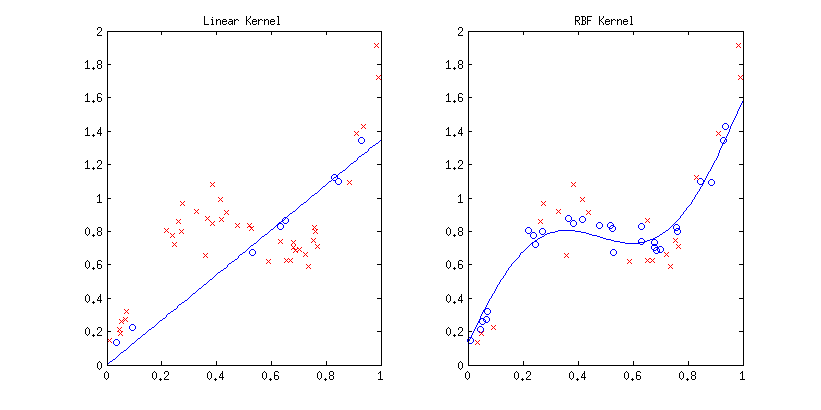
\includegraphics[trim=22mm 5mm 21mm 4mm, clip=true, width=0.64\linewidth]{1_1_4}
\vspace{-6mm}
\caption{$\hat f$ as predicted by support vector regression using linear and
RBF kernels. Support vectors are indicated by crosses.}
\label{fig:1_1_4}
\end{figure}
\end{enumerate}
\subsubsection*{Code}
\begin{verbatim}
function [params, svs] = dualSVMRegression(K, y, c, eps)

  n = length(y);
  z = [eps - y', eps + y'];
  Q = [K -K; -K K];

  theta = quadprog(Q, z, [], [], [], [], zeros(2*n,1), c*ones(2*n,1));

  params.beta = theta(1:n);
  params.gamma = theta((n + 1):end);
  svs = abs(params.beta - params.gamma) > 0.01;

end

function preds = dualSVMPredict(params, ks)
  preds = (params.beta - params.gamma)'*ks;
end

function K = rbfKernel(X1, X2, h)

  n1 = length(X1);
  n2 = length(X2);
  K = zeros(n1,n2);
  for i=1:n1
    for j=1:n2
      K(i,j) = exp(-(X1(i) - X2(j))^2/(2*h^2));
    end
  end
end
\end{verbatim}
\newpage
\section{Expectation Maximization (Samy)}
\subsection{EM Basics}
\begin{enumerate}
\item For any probability density $q$, since $P(y,D | \theta^t) = P(D | \theta^t)P(y | D,\theta^t)$,
\begin{align*}
\log P(D | \theta^t)
 &  = \int q(y) \log P(D | \theta^t) \, dy
    = \int q(y) \log \frac{P(y,D | \theta^t)q(y)}{P(y | D,\theta^tq(y)} \, dy\\
 &  = \int q(y) \log P(y,D | \theta^t) \, dy
    + \int q(y) \log \frac1{q(y)} \, dy
    + \int q(y) \log \frac{q(y)}{P(y | D,\theta^t)} \, dy\\
 &  = \int q(y) \log P(y,D | \theta^t) \, dy + H(q) + D_{KL}(q(y) \| P(y | D,\theta^t)),
\end{align*}
where $H$ denotes Shannon entropy and $D_{KL}$ denotes KL-divergence. Since $H$
and $D_{KL}$ are nonnegative, in the case $q(y) = P(y | D,\theta^t)$,
\[\log P(D | \theta^t)
    \geq \int P(y | D,\theta^t) \log P(y,D | \theta^t) \, dy
    = Q(\theta | \theta^t),
\]
where $Q(\theta | \theta^t)$ is the expression we maximize in the M-step. \qed
\item Since $\theta^{t + 1} := \arg\!\max_{\theta} Q(\theta | \theta^t)$ and
$D_{KL}(p || q) \geq 0$ with equality if $p = q$,
\begin{align*}
\log P(D | \theta^t)
 &  = Q(\theta^t | \theta^t) + H(P(y | D,\theta^t)) + D_{KL}(P(y | D,\theta^t) \| P(y | D,\theta^t)) \\
 &  \leq Q(\theta^{t + 1} | \theta^t) + H(P(y | D,\theta^t)) + D_{KL}(P(y | D,\theta^{t + 1}) \| P(y | D,\theta^t)) \\
 &  = \log P(D | \theta^{t + 1}). \qed
\end{align*}
\end{enumerate}

\subsection{P\'olya Mixture Model}
\subsubsection{Model}
As shown in HW 1, for any labels $z_1,\dots,z_n$ the log-joint probability is
\begin{align*}
 & \ell(x_1,\dots,x_n,z_1,\dots,z_n,\theta,\alpha_1,\dots,\alpha_K) \\
 &  = \sum_{j = 1}^K (\theta_0^{(j)} - 1)\log\theta^{(j)}
                        - \lambda\|\alpha_j\|^2
    + \sum_{i = 1}^n 1_{\{z_i = j\}}
                \left( \log\theta^{(j)} + \log p_{dm}(x_i; \alpha_j) \right)
    + C(\theta_0,\lambda),
\end{align*}
where $C$ is constant in $x_i$'s, $z_i$'s, $\theta$, and $\alpha_j$'s. I didn't
have time to write out the derivation.

In the E-step, we predict $z_1,\dots,z_n$ using the previous value of $\theta$
and $\alpha_1,\dots,\alpha_k$. In the M-step, we update our estimates of
$\theta$ and $\alpha_1,\dots,\alpha_k$ using the labels $z_1,\dots,z_n$. Both
prediction of $z_1,\dots,z_n$ and estimation of $\theta$ and
$\alpha1,\dots,\alpha_K$ are performed as in Homework 1. Our prediction rule is
the MAP estimate
\[z_*
    = \arg\!\max_{j \in \{1,\dots,K\}} p(z = j | x_*)
    = \arg\!\max_{j \in \{1,\dots,K\}} p(x_* | z = j)p(z = j)
    = \arg\!\max_{j \in \{1,\dots,K\}} p_{dm}(x_*;\hat\alpha_j)\hat\theta^{(j)},
\]
where $\hat\theta$ and $\hat\alpha_1,\dots,\hat\alpha_K$ are as predicted by
our EM procedure.

\subsubsection{Experiment}
\begin{verbatim}
>> q22

theta =

    0.3003
    0.4532
    0.2465

alpha =

    0.3658    0.2736    0.3919    0.2659    0.3302
    0.2915    0.2626    0.3893    0.2735    0.3887
    0.4732    0.3347    0.2665    0.5032    0.4318

preds =

     1
     1
     3
     1
     2
Accuracy: 99.1300
\end{verbatim}

\newpage
\subsubsection*{Code}
\begin{verbatim}
function [theta, alpha] = trainPMM(XTrain, K, theta0, lambda, thetaInit, alphaInit);

  theta = thetaInit;
  alpha = alphaInit;

  for iter = 1:10
    Z = predictPMM(XTrain, theta, alpha);
    [theta, alpha] = trainPDA(XTrain, Z, theta0, lambda);
  end
end

function [theta, alpha] = trainPDA(X, y, theta0, lambda)

  % Prelims
  K = numel(unique(y));
  V = size(X, 2);
  numData = size(X, 1);

  % MAP for theta
  table = tabulate(y);
  adjustedFreqs = table(:,2) + theta0 - 1;
  theta = adjustedFreqs/sum(adjustedFreqs);

  % MAP for alpha
  alpha = zeros(K, V);
  parfor k = 1:K
    Xk = X(y == k, :);
    alpha(k, :) = newtonRaphsonPDA(Xk, lambda);
  end
end

function [alpha_k] = newtonRaphsonPDA(Xk, lambda)

  % Prelims
  numNRIters = 10; % Just use 5 iterations of NR
  nk = size(Xk, 1); % number of training data in this class
  m = sum(Xk, 2); % number of words in each documents
  initPt = sum(Xk); initPt = initPt/sum(initPt); % Initialization

  % Now perform Newton's
  alpha_k = initPt; % alphak in the current iteration
  for nrIter = 1:numNRIters
    % Compute the following
    Ak = sum(alpha_k);
    XplusAlpha = bsxfun(@plus, Xk, alpha_k);
    % The gradient
    g = nk * psi(Ak) - sum(psi(m + Ak)) + sum( psi(XplusAlpha) ) ...
        - nk * psi(alpha_k) - 2 * lambda * alpha_k;
    % The value z (see solutions)
    z = nk * psi(1, Ak) - sum(psi(1, m + Ak));
    % The diagonal of the Hessian
    D = sum(psi(1, XplusAlpha)) - nk * psi(1, alpha_k) - 2*lambda;
    % Newton's step update
    Hinvg = g./D - (1./D) * sum(g./D) / (1/z + sum(1./D));
    alpha_k = alpha_k - 1*Hinvg;
  end
end

function [preds, classLogJoints] = predictPMM(X, theta, alpha)

  % prelims
  n = size(X, 1);
  K = numel(theta);

  % First obtain the class log joint probabilities
  classLogLs = zeros(n, K);
  parfor k = 1:K
    classLogLs(:, k) = classLogLikelihoods(X, alpha(k, :));
  end
  classLogJoints = bsxfun(@plus, classLogLs, log(theta'));

  % Finally obtain the predictions
  [~, preds] = max(classLogJoints, [], 2);

end

function logL = classLogLikelihoods(X, alphak)

  % Prelims
  Ak = sum(alphak);
  m = sum(X, 2); % number of words in each documents
  XplusAlpha = bsxfun(@plus, X, alphak);

  % Compute the log likelihood
  logL = gammaln(Ak) - gammaln(m + Ak) + ...
    sum(gammaln(XplusAlpha), 2) - sum( gammaln(alphak) );
end
\end{verbatim}
\newpage


\newpage
\setcounter{footnote}{0}
{\Large Homework \myhwnum, Problems 3 and 4} \\
Name: \myname \\
\myclass \\
Due: \duedate

\section{Kernels and RKHS (Veeru)}
\subsection{Image Similarity Functions}
\begin{enumerate}
\item Consider a set $I$ indexing the set of $16 \times 16$ pixel patches.
Then, $k_1(x,x') = \sum_{i \in I} k_i$
where $k_i(x,x') = 0$ when either $x$ or $x'$ has no $i^{th}$ patch or when
their $i^{th}$ patches are different, and $k_i(x,x') = 1$ otherwise. Since each
$k_i$ is trivially a positive definite kernel (specifically, a $\delta$
function), it follows from part 1 of section 3.2 below that $k_1$ is a positive
definite kernel. \qed
\item Consider three $16 \times 32$ images $A,B,C \in X$, where $A$ is entirely
black, $B$ is black on the left half and white on the right half, and $C$ is
white on the left half and black on the right half. Then, the kernel matrix of
$k_2$ evaluated on $A,B,C$ is
\[K =
\begin{bmatrix}
  1 & 1 & 1 \\
  1 & 1 & 0 \\
  1 & 0 & 1 \\
\end{bmatrix}.
\]
It can be checked that $K$ has an eigenvalue of $\approx -0.41$, and hence $K$
is not positive semidefinite. \qed
\end{enumerate}

\subsection{Positive definiteness of Gaussian Kernel}
\begin{enumerate}
\item By Mercer's Theorem, it suffices to observe that,
$\forall f \in L^2(\R^d)$,
\begin{align*}
&\hspace{-10mm}
\int_{\R^d} \int_{\R^d} (\alpha k_1 + \beta k_2)(x,y) f(x) f(y) \, dy \, dx\\
 &  = \alpha \int_{\R^d} \int_{\R^d} k_1(x,y) f(x) f(y) \, dy \, dx
    + \beta \int_{\R^d} \int_{\R^d} k_2(x,y) f(x) f(y) \, dy \, dx
    \geq 0. \qed
\end{align*}
\item Suppose $x_1,\dots,x_n$ are in the domain of $k_1$ and $k_2$. Let
$K_1,K_2 \in \R^{n \times n}$ denote the kernel matrices under $k_1,k_2$,
respectively. Since $K_1,K_2$ are positive-semidefinite, they have
positive-semidefinite square roots $A,B \in \R^{n \times n}$ with $A^2 = K_1$
and $B^2 = K_2$. Let $K := K_1 \circ K_2$ and note that, since $K$ is the
kernel under $k_1k_2$, it suffices to show $K$ is positive-semidefinite. Note
that, for $i,j \in [n]$,
\[K_{i,j}
    = (K_1)_{i,j}(K_2)_{i,j}
    = \left( \sum_{k = 1}^n A_{i,k}A_{j,k} \right)
    \left( \sum_{\ell = 1}^n B_{i,\ell}B_{j,\ell} \right).
\]
Thus, for any $y \in \R^n$,
\begin{align*}
y^TKy
 &  = \sum_{i = 1}^n \sum_{j = 1}^n y_iy_j
    \left( \sum_{k = 1}^n A_{i,k}A_{j,k} \right)
    \left( \sum_{\ell = 1}^n B_{i,\ell}B_{j,\ell} \right)   \\
 &  = \sum_{k = 1}^n \sum_{\ell = 1}^n
    \left( \sum_{i = 1}^n y_iA_{i,k}B_{i,\ell} \right)
    \left( \sum_{j = 1}^n y_jA_{j,k}B_{j,\ell} \right)  \\
 &  = \sum_{k = 1}^n \sum_{\ell = 1}^n
    \left( \sum_{i = 1}^n y_iA_{i,k}B_{i,\ell} \right)^2
    \geq 0. \qed
\end{align*}

\item For $x_1,\dots,x_n \in \R^d$, $y \in \R^n$, Taylor-expanding the
exponential function,
\begin{align*}
\sum_{i = 1}^n \sum_{j = 1}^n \exp(k(x_i,x_j)) y_iy_j
    = \sum_{\ell = 0}^\infty \sum_{i = 1}^n \sum_{j = 1}^n
            \frac{k^\ell(x_i,x_j)}{\ell!} y_iy_j
    \geq 0,
\end{align*}
since $k^\ell$ is a kernel. \qed
\item Any real inner product is a kernel, since,
$\forall x_1,\dots,x_n$ in the appropriate domain, $y \in \R^n$,
\[\sum_{i = 1}^n \sum_{j = 1}^n \langle x_i, x_j \rangle y_i y_j
    = \sum_{i = 1}^n \left\langle y_i x_i, \sum_{j = 1}^n y_j x_j \right\rangle
    = \left\langle \sum_{i = 1}^n y_i x_i, \sum_{j = 1}^n y_j x_j \right\rangle
    = \left\| \sum_{i = 1}^n y_i x_i \right\|_{\langle \cdot, \cdot \rangle}^2
    \geq 0.
\]
Hence, since the function $(x_1,x_2) \mapsto \delta x_1^Tx_2$ is an inner
product on $\R^d$, by the previous part, the function
$(x_1,x_2) \mapsto \exp(2\delta x_1^Tx_2)$ is a kernel. Since the function
$(x_1,x_2) \mapsto \exp(-\delta(\|x_1\|_2^2 + \|x_2\|_2^2))$ is also a kernel
(I didn't have time to show this), their product, the Gaussian kernel, is a
positive definite kernel. \qed

\item Let $x,y \in \R^d$ with $x \neq y$. Since $k(x,\cdot) \neq k(y,\cdot)$,
it follows that $2k(x,y) < k(x,x) + k(y,y)$, and hence
$\exp(-(k(x,x) + k(y,y))) - \exp(-2k(x,y)) < 0$. This expression is the
determinant of the $2 \times 2$ kernel matrix for $x,y$ under $\exp(-k)$, and
hence this matrix is not positive-semidefinite (a positive-semidefinite matrix
clearly has nonnegative determinant). \qed
\end{enumerate}

\subsection{Checking validity by Fourier transforms}
\begin{enumerate}
\item For $\omega \in \R$, completing the square in the argument of $\exp$,
\begin{align*}
\F[k'](\omega)
 &  = \frac{1}{\sqrt{2\pi}} \int_\R e^{-i\omega x} e^{-\delta x^2} \, dx    \\
 &  = \frac{1}{\sqrt{2\pi}} \int_\R
                        \exp \left( -(\delta x^2 + i\omega x) \right) \, dx \\
 &  = \frac{1}{\sqrt{2\pi}} \int_\R \exp \left(
        -\left( \sqrt{\delta} x + \frac{i\omega}{2\sqrt{\delta}} \right)^2
    - \omega/(4\delta)
        \right) \, dx \\
 &  = \frac{\sqrt{1/\delta}\exp(-\omega/(4\delta))}{\sqrt{2\pi/\delta}}
            \int_\R \exp \left(
                -\frac{\left( x + i\omega/2 \right)^2}{2/\delta}
            \right) \, dx
    = \frac{\exp(-\omega/(4\delta))}{\sqrt{\delta}}
    > 0,
\end{align*}
where we used the fact that the integral over $\R$ of the pdf of
$\mathcal{N}(-i\omega/2,1/\delta)$ is $1$. \qed

\item Define $\hat k : \R \to \R$ by
$\hat k(\omega) = \sqrt{\pi/2} e^{-|\omega|}$, for all $\omega \in \R$. Then,
$\forall x \in \R$,
\begin{align*}
\F\left[ \hat k \right](x)
    = \frac{1}{2} \int_\R e^{-(ix\omega + |\omega|)} \, d\omega
 &  = \frac{1}{2} \left( \int_0^\infty e^{-(1 + ix)\omega} \, d\omega
    + \int_0^\infty e^{-(1 - ix)\omega} \, d\omega \right)  \\
 &  = \frac{1}{2} \left( \frac{1}{1 + ix} + \frac{1}{1 - ix} \right)
    = \frac{1}{1 + x^2}
    = k'(x).
\end{align*}
Since $\hat k$ is even and $\F^2$ is the time-reversing function,
$\F[k'] = \F^2 \left[ \hat k \right] = \hat k > 0$. \qed
\end{enumerate}

\subsection{RKHS from the eigenfunctions of the kernel's integral operator}
Let $f \in \mathcal{H}_k, x \in X$. Since $\{\phi_i\}_{i = 1}^\infty$ is a
basis for $\mathcal{H}_k$, $\exists !\{f_i\}_{i = 1}^\infty \in \R^\N$ such that
$f = \sum_{i = 1}^\infty f_i \phi_i$. Then,
\[f(x)
    = \sum_{i = 1}^\infty f_i \phi_i(x)
    = \sum_{i = 1}^\infty \frac{f_i \lambda_i \phi_i(x)}{\lambda_i}
    = \langle f, k(\cdot,x) \rangle. \qed
\]

\subsection{Optimizing over an RKHS}
Define a subspace $\H_{||} \subseteq \H_k$ by
$\H_{||} := \left\{ \sum_{i = 1}^n \alpha_i k(\cdot, x_i)
                                                    : \alpha \in \R^n \right\}
$. Since $\H_{||}$ is finite dimensional and hence closed, for any
$f \in \H_k$, we can define $f_{||} \in \H_{||}$ as the unique projection of
$f$ onto $\H_{||}$, and define $f_\perp \in \H_k$ by $f_\perp := f - f_{||}$.
Then, for each $i \in [n]$,
\begin{align*}
(y_i - f(x_i))^2
    = (y_i - \langle f, k(\cdot,x_i) \rangle)^2
    = (y_i - \langle f_{||}, k(\cdot,x_i) \rangle)^2
    = (y_i - f_{||}(x_i))^2
\end{align*}
and, by the Pythagorean Theorem,
$\|f\|_{\H_k}^2 = \|f_{||}\|_{\H_k}^2 + \|f_\perp\|_{\H_k}^2$. Hence
\[\sum_{i = 1}^n (y_i - f(x_i))^2 + \lambda\|f\|_{\H_k}^2
    \geq \sum_{i = 1}^n (y_i - f_{||}(x_i))^2 + \lambda\|f_{||}\|_{\H_k}^2,
\]
and so any minimizer $f_*$ of $(2)$ has the form
$f_* = \sum_{i = 1}^n \alpha_i k(\cdot,x_i), \alpha \in \R^n$. So, $(2$) is
equivalent to
\begin{equation*}
\min_{\alpha \in \R^n}
    \sum_{i = 1}^n
        \left( y_i - \sum_{j = 1}^n \alpha_i k(x_j,x_i) \right)^2
    + \lambda\left\|\sum_{i = 1}^n \alpha_i k(\cdot, x_i) \right\|_{\H_k}.
\end{equation*}
By the reproducing property,
\[\left\|\sum_{i = 1}^n \alpha_i k(\cdot, x_i) \right\|_{\H_k}
    = \sum_{i = 1}^n \sum_{j = 1}^n \alpha_i\alpha_j
                                    \langle k(\cdot,x_i), k(\cdot,x_j) \rangle
    = \sum_{i = 1}^n \sum_{j = 1}^n \alpha_i\alpha_j k(x_i,x_j)
    = \alpha^T K \alpha,
\]
where $K$ denotes the kernel matrix of $k$ evaluated on $x_1,\dots,x_n$. Also,
\[\sum_{i = 1}^n \left( y_i - \sum_{j = 1}^n \alpha_i k(x_j,x_i) \right)^2
    = \|K\alpha - y\|_2^2.
\]
Hence the problem can be rewritten as
\[\min_{\alpha \in \R^n} \|K\alpha - y\|_2^2 + \lambda\alpha^T K \alpha.\]
If $\hat\alpha$ minimizes this, then
\[0
    = \nabla_\alpha \|K\alpha - y\|_2^2
                        + \lambda\alpha^T K \alpha \big|_{\alpha = \hat\alpha}
    = K(K\hat\alpha - y) + \lambda K \alpha
    = (K^2 + \lambda K) \hat\alpha - Ky.
\]
As long as $K$ is nonsingular, solving for $\hat\alpha$ gives and hence
\fbox{$\hat\alpha = (K + \lambda I)\inv y$} (noting that $K + \lambda I$ is
nonsingular, since $K$ has only nonnegative eigenvalues).

\subsection{Some computational considerations for SVM}
\begin{enumerate}
\item Naively implementing kernel SVM requires storing the $m \times m$ kernel
matrix of $x_1,\dots,x_m$. Hence, the space complexity is $O(m^2)$.
\item Since the decision function requires computing the kernel $k(x,x_i)$ for
each support vector $x_i$, this takes $O(md)$ time.
\item The Fastfood approach proposed by Le et al. takes $O(m \log d)$ time and
$O(n)$ storage.
\end{enumerate}

\end{document}
